\textbf{5-1}已知冕牌玻璃k9的折射率遵从下述科希公式，
$$ n = A + \frac {B}{\lambda^ {2}} + \frac {C}{\lambda^ {4}} $$
式中 $A = 1.504, B = 4.437 \times 10^{3} \mathrm{~nm}^{2}, C = -1.387 \times 10^{8} \mathrm{~nm}^{4}$ . 试求该玻璃对钠黄色双线的相速和群速. 已知双线的平均波长为 $589.3 \mathrm{~nm}$ , 冕牌玻璃对该波长的折射率为 1.51630.
\vfill

\textbf{5-2}已知氢的电子吸收谱位于远紫外波段，常温常压下氢在 $0.4\mu \mathrm{m}$ 到 $9\mu \mathrm{m}$ 波段的折射率遵从下述经验公式，

$$ n ^ {2} = 1 + 2. 7 2 1 \times 1 0 ^ {- 4} + \frac {2 . 1 1 \times 1 0 ^ {- 1 8}}{\lambda^ {2}} $$

式中波长 $\lambda$ 以米(m)为单位.

试利用塞耳迈耶尔色散公式求:

1. 氢原子的本征频率和相应的共振吸收波长 .

2. 振子的荷质比,已知氢的密度为 $9.0 \times 10^{-2} \, kg/m^{3}$ .
\vfill

\newpage
\textbf{5-3}已知 $\mathrm{CaF}_2$ 在 $0.3\mu \mathrm{m}$ 到 $10~\mu \mathrm{m}$ 波长范围内的折射率的经验公式为
$$ n ^ {2} = 6. 0 9 + \frac {6 . 1 2 \times 1 0 ^ {- 1 5}}{\lambda^ {2} - 8 . 8 8 \times 1 0 ^ {- 1 5}} + \frac {5 . 1 0 \times 1 0 ^ {- 9}}{\lambda^ {2} - 1 . 2 6 \times 1 0 ^ {- 9}} $$
式中波长 $\lambda$ 的单位是米(m).试求:

1. $CaF_{2}$ 吸收谱的波长.

2. 根据所给数据估算质子和电子的质量比.已知 F 的原子量为 19,Ca 的原子量为 40.
\vfill

\textbf{5-4}1. 试证明，在X射线波段，物质的色散规律为
$$ n ^ {2} = 1 - K \lambda^ {2} $$
式中 $\lambda$ 为 X 射线在真空中的波长，K 为与电子数密度有关的系数。试求铜的 K 值，已知铜的原子序数 Z=29，原子量 A=63，密度 $\rho=8\times10^{3}\ kg/m^{3}$ 。

2. 试证明, X 射线在物质中的相速 $v_{p}$ 和群速 $v_{g}$ 遵从下述关系
$$ v _ {p} v _ {g} = c ^ {2} $$
式中 $c$ 为真空中的光速.
\vfill

\newpage
\textbf{5-5}假设对金属光学性质有影响的是价电子.

1.试导出在弱阻尼情形下金属的色散关系.

2.试求正入射时能量反射率与波长的关系.
\vfill

\textbf{5-6}大气上层的电离层可看作是由正离子和负电子构成的等离子体，假定电离层与非电离的大气层具有一截然分开的界面。

1. 设电磁波的频率 $\nu = 2\nu_{p}$ 或 $\nu \ll \nu_{p}$ . 当电磁波从大气一侧向上述分界面正入射时, 试计算这两种情形的能量反射率. 其中 $\nu_{p}$ 为等离子体振荡频率. 

2. 当电磁波从大气一侧入射到上述分界面时, 为使反射的电磁波中只包含垂直于入射面的振动, 试问入射角应为何值?
\vfill

\newpage
\textbf{5-7}试先就一般的各向同性介质，讨论麦克斯韦方程组具有平面纵波解的条件。然后将此条件应用于等离子体，试讨论所得结论的含义。
\vfill

\textbf{5-8}试根据经典电磁理论，证明无密度涨落的均匀介质对光无散射。介质的任何不均匀性，将导致各散射中心发出的次波振幅的不一致，设振幅涨落为 $\Delta A$ ，试证明散射光强度与 $\Delta A$ 的方均值成正比.
\vfill

\newpage
\textbf{5-9}根据经典电磁理论，试证明由散射物质的密度涨落所引起的散射光光强遵守瑞利散射公式，即散射角为 $\theta$ 处的散射光强为
$$ I _ {\theta} \propto \frac {1 + \cos^ {2} \theta}{\lambda^ {4}} $$
式中 $\lambda$ 为入射光的波长. 已知介质的相对电容率(介电常量) $\varepsilon_r$ 与密度 $\rho$ 有关, 且 $\frac{\partial \varepsilon_r}{\partial \rho}$ 保持恒定, $\varepsilon_r$ 与温度 $T$ 的依赖关系可略.

提示:如光图5-9-1所示,把散射介质分成许多小体积元,小体积的线度比波长小得多,每个体积元可看作是一电偶极子,设其电偶极矩为p.观察点的经矢为r,r与p的夹角为 $\alpha$ .当观察点离电偶极子足够远时,偶极发射的电场强度由下式决定,
$$ E _ {\alpha} = \frac {\omega^ {2} p}{4 \pi \varepsilon_ {0} c ^ {2} r} \sin \alpha $$
各偶极发射的相干叠加构成了某方向上的散射光。

\begin{center}
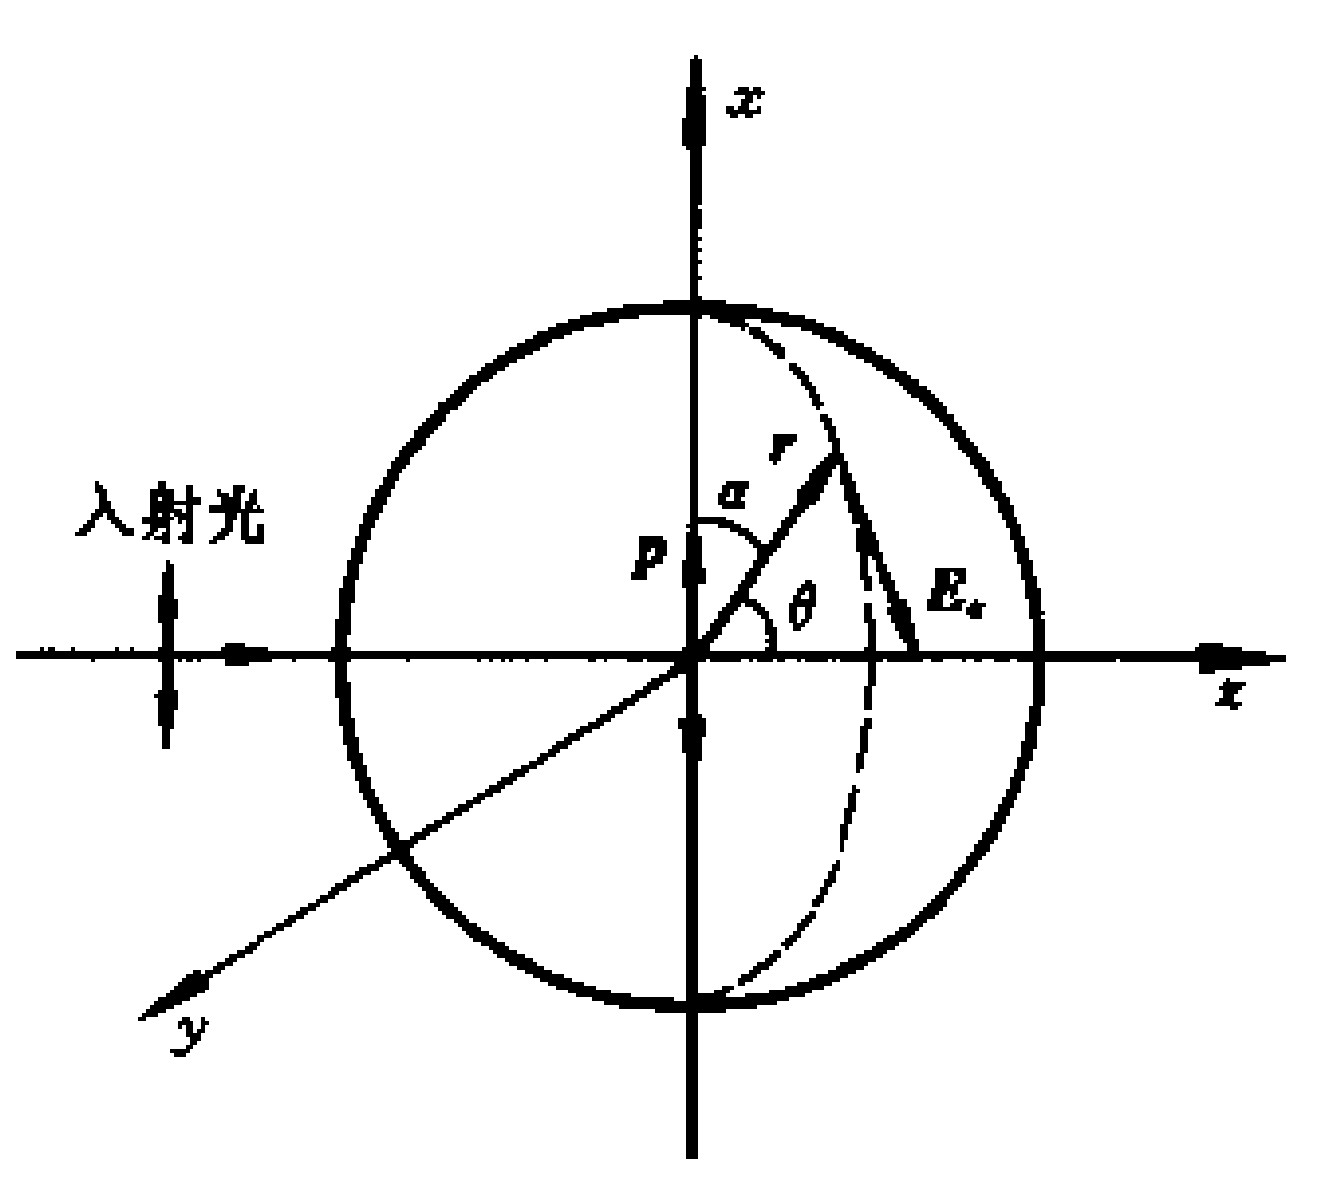
\includegraphics[width=0.3\textwidth]{figures/光图5-9-1.jpg}
\end{center}

\vfill\newpage

\textbf{5-10}空间一射电源发出一宽频带的“噪音”脉冲。由于在星际介质中的色散，这一脉冲到达地球时，就变成频率随时间变化的哨声。若哨声的频率改变率 $\frac{\mathrm{d}\omega}{\mathrm{d}t}$ 已被测出，并且地球与射电源的距离 $L$ 是已知的，就可以推出星际介质中电子的平均密度 $N$ 。试导出决定 $N$ 的公式。假定星际介质是完全电离的，即为等离子体。
\vfill



\vfill

\textbf{5-11} 强度为 $I_0$ 的单色光垂直入射到有色玻璃片上，玻璃片的厚度为 $l$ ，吸收系数为 $\alpha$ ，折射率 $n = 1.5$ 。1. 试求透射光强和入射光强之比(不计多重反射)。2. 试求由于不计光强的反射损失而引起的相对误差是多少？假设能量反射率 $R$ 很小。3. 试问在测量玻璃片的吸收系数 $\alpha$ 的实验中，怎样消除由于反射引起的误差？

\vfill
